\documentclass[a4paper]{report}

\usepackage{mythesis}

% Graphics directory
\graphicspath{{img/}}

% Title page options
\title{\thesisTitle{}}
\author{\studentName{}}
\date{\thesisDate{}}

% Bibliography
\bibliography{thesis}

%%%%%%%%%%%%%%%%%%%%%%%%%%%%%%%%%%%%%%%%%%%%%%%%%%%%%%%%%%%%%%%%%%%%%%%%%%%%%%%%

\begin{document}

%%%%%%%%%%%%%%%%%%%%%%%%%%%%%%%%%%%%%%%%%%%%%%%%%
% Title Page
%%%%%%%%%%%%%%%%%%%%%%%%%%%%%%%%%%%%%%%%%%%%%%%%%
\begin{titlepage}
\begin{center}

% Upper part of the page

\includegraphics[width=0.25\textwidth]{sydney_uni_coat_of_arms}\\[1cm]

\textsc{\LARGE \universityName{}}\\[1.5cm]

\textsc{\Large Final year thesis}\\[0.5cm]

% Title
\HRule \\[0.4cm]
{\huge \bfseries \thesisTitle{}}\\[0.4cm]
\HRule \\[1.5cm]

% Author and supervisor
\begin{minipage}{0.4\textwidth}
    \begin{flushleft} \large
        \emph{Author:}\\
        \studentName{}
    \end{flushleft}
\end{minipage}
\begin{minipage}{0.4\textwidth}
    \begin{flushright} \large
        \emph{Supervisor:} \\
        \supervisorName{}
    \end{flushright}
\end{minipage}

% strech vertical space so that it fills all empty space
\vfill

% Thesis description
{\large A thesis submitted in fulfilment of the requirements for the\\
degree of Bachelor of Engineering (Computer) in the \\
School of Electrical Engineering at\\
The University of Sydney}

% strech vertical space so that it fills all empty space
\vfill

% Bottom of the page
{\large \thesisDate{}}

\end{center}
\end{titlepage}

\pagenumbering{roman}

%%%%%%%%%%%%%%%%%%%%%%%%%%%%%%%%%%%%%%%%%%%%%%%%%
% Acknowledgements
%%%%%%%%%%%%%%%%%%%%%%%%%%%%%%%%%%%%%%%%%%%%%%%%%
\chapter*{Acknowledgements}
This project could not be completed without the guidance of my project 
supervisor, \supervisorName{}. He always made himself available to assist me 
with the understanding of many new and unknown concepts. His expertise in the 
field was a great asset and greatly contributed to my own understanding of the 
ideas explored in this thesis. His support and guidance was invaluable, and were
instrumental to the success of my project. 

Additionally, much of the works completed during this project could not have 
been performed without the prior research of \contributorOne{} and 
\contributorTwo{}. Both were generous enough to lend their own support and 
expertise in order to gain an understanding of the implemented random projection
algorithms.

%%%%%%%%%%%%%%%%%%%%%%%%%%%%%%%%%%%%%%%%%%%%%%%%%
%  Publications
%%%%%%%%%%%%%%%%%%%%%%%%%%%%%%%%%%%%%%%%%%%%%%%%%
\chapter*{Publications}
This thesis is based on the following publications:
\begin{enumerate}
\item \fullcite{Vries:2010}
\item \fullcite{Khoa:2012}
\item \fullcite{Bay:2003}
\end{enumerate}

%%%%%%%%%%%%%%%%%%%%%%%%%%%%%%%%%%%%%%%%%%%%%%%%%
% Abstract
%%%%%%%%%%%%%%%%%%%%%%%%%%%%%%%%%%%%%%%%%%%%%%%%%
\begin{abstract}
The prediction of the stock market has become an issue of great interest in the
areas of finance, mathematics and engineering; due mainly to the great potential
financial gain. Researchers have devised various algorithms and differing 
approaches to the problem of stock market analysis, with varying degrees of 
success.

A major outstanding issue for stock market analysis is the effective and 
efficient detection of local anomalies in the input data sets, which are 
inherently highly multidimensional. Many na\"{\i}ve algorithms are highly 
inefficient and others fail to adequately detect local anomalies altogether. It
had become a time-vs-correctness trade-off in which no acceptable compromise
could be reached.

However, researchers are starting to explore the relatively new concept of 
applying ``random projections'' to the highly multidimensional data sets. 
Research has suggested that by applying these random projections, they are able 
to significantly reduce the dimensionality (and consequently the computational 
complexity) of the data sets, whilst sufficiently retaining the inherent 
properties of that data set --- at least so much so as anomaly detection is 
concerned.

Anomaly detection is important because it allows otherwise-accurate machine 
learning algorithms such as neural networks to more accurately model and predict
the stock exchange data by ignoring anomaly data, which likely doesn't effect 
the state of the model to any significant degree.

\contributorOne{} from the ``University of Sydney'' has in recent years 
conducted and supervised new and exciting research oriented around random 
projections. In particular, \contributorTwo{}, under the supervision of 
\contributorOne{} evaluated the use of traditional distance metrics, such as 
Euclidean distance and Mahalanobis distance, in the application of local anomaly
detection. \contributorTwo{} proposed the use of the `commute time' metric, 
derived from random walks on graphs, in anomaly detection.
\end{abstract}

%%%%%%%%%%%%%%%%%%%%%%%%%%%%%%%%%%%%%%%%%%%%%%%%%
% Table of Contents
%%%%%%%%%%%%%%%%%%%%%%%%%%%%%%%%%%%%%%%%%%%%%%%%%
\tableofcontents

%%%%%%%%%%%%%%%%%%%%%%%%%%%%%%%%%%%%%%%%%%%%%%%%%
% List of Figures
%%%%%%%%%%%%%%%%%%%%%%%%%%%%%%%%%%%%%%%%%%%%%%%%%
\listoffigures

%%%%%%%%%%%%%%%%%%%%%%%%%%%%%%%%%%%%%%%%%%%%%%%%%
% List of Algorithms
%%%%%%%%%%%%%%%%%%%%%%%%%%%%%%%%%%%%%%%%%%%%%%%%%
\listofalgorithms

%%%%%%%%%%%%%%%%%%%%%%%%%%%%%%%%%%%%%%%%%%%%%%%%%
% List of Tables
%%%%%%%%%%%%%%%%%%%%%%%%%%%%%%%%%%%%%%%%%%%%%%%%%
\listoftables

\pagenumbering{arabic}

%%%%%%%%%%%%%%%%%%%%%%%%%%%%%%%%%%%%%%%%%%%%%%%%%
% CHAPTER 01: Introduction
%%%%%%%%%%%%%%%%%%%%%%%%%%%%%%%%%%%%%%%%%%%%%%%%%
\chapter{Introduction}
\label{ch:intro}

\section{Motivation}
\label{sec:motivation}
Anomaly detection is an important technique which can be applied to a wide 
range of applications. There are many techniques to detect and measure 
anomalies, each usually most applicable to some specific problem domain. A 
general algorithm for anomaly detection has proved difficult to design, due to 
various challenges associated with defining and measuring anomalies. Most 
existing approaches are based on statistical or geometrical measures involving 
distance. Whilst many algorithms work well for some subset of input data sets, 
it has been difficult to discover an algorithm which performs both correctly and
efficiently on all possible data sets.

Previous research has found merit in applying randomization techniques to highly
multivariate data sets in order to reduce the dimensionality of these data sets 
whilst maintaining their fundamental and statistical properties. Such reduction 
of the dimensionality of data, assuming it can be performed efficiently, allows 
previously-unscalable anomaly detection algorithms to be practically applied to 
a wider range of data and applications.

Anomaly detection is an important and contemporary problem in the field of 
computer science, and is of particular interesting to stock market analysis, 
network intrusion detection and image comparison.


\section{Contributions of this thesis}
\label{sec:contributions}
One key difficulty in anomaly detection is the efficient scaling of a general 
algorithm to apply to highly multivariate data. In this thesis, I explore the 
use of randomization techniques (such as random projections and commute time) 
in anomaly detection algorithms. These techniques provide encouraging results 
with regards to the run-time complexity of an algorithm.

Furthermore, in this thesis I attempt to make observations and analysis of the 
run-time of anomaly detection using randomization techniques, so as to identify
steps in the algorithms that bottleneck the algorithm's performance. Through 
this identification it would be possible to improve the \emph{actual} run-time 
performance of the algorithm by utilisation the advantages of reconfigurable 
computing.


\section{Organization}
\label{sec:organization}
The rest of this thesis is organized as follows. In \hyperref[ch:background]
{Chapter~\ref{ch:background}}, we provide background to various anomaly 
detection techniques, as well as randomization techniques. In order to provide 
the reader with an understanding of the background topics, a brief background is
given to various topics in linear algebra, vector calculus and graph theory. In
\hyperref[ch:reconfigurableComputing]{Chapter~\ref{ch:reconfigurableComputing}}, 
we provide an overview of reconfigurable computing, including an explanation of 
Field-Programmable Gate Arrays (FPGAs).

In \hyperref[ch:design] {Chapter~\ref{ch:design}}, we profile the execution of 
an anomaly detection algorithm and explore possible improvements to the 
algorithm, in particular by outsourcing various stages of the algorithm to an 
FPGA device. In \hyperref[ch:implementation]{Chapter~\ref{ch:implementation}}, 
we describe the implementation of the improved algorithm and detail the process 
that was followed in order to construct the hardware processing device. In 
\hyperref[ch:results]{Chapter~\ref{ch:results}}, we record results obtained by 
benchmarking the device that was previously designed and constructed, and 
comparing the expected improvements to the algorithm's execution with the 
measured results.

We conclude in \hyperref[ch:conclusions] {Chapter~\ref{ch:conclusions}} by 
reflecting upon the results obtained through this research, and making 
suggestions for further research in this topic.

 
\section{Schedule}
\label{sec:schedule}
A Gantt chart showing the anticipated schedule for the project is shown in 
\autoref{fig:ganttChart}. This will be updated as the project progresses.

% Gantt chart
% See http://www.martin-kumm.de/tex_gantt_package.php
\begin{figure}[h]
	\centering
	\scalebox{0.5}{
	\begin{gantt}[
			xunitlength=0.5cm,
			fontsize=\small,
			titlefontsize=\small,
			drawledgerline=true
			]{18}{36}
		% Months
		\begin{ganttitle}
			\titleelement{Mar}{4}
			\titleelement{Apr}{4}
			\titleelement{May}{4}
			\titleelement{Jun}{4}
			\titleelement{Jul}{4}
			\titleelement{Aug}{4}
			\titleelement{Sep}{4}
			\titleelement{Oct}{4}
			\titleelement{Nov}{4}
		\end{ganttitle}
		% Split months into quarters
		\begin{ganttitle}
			\numtitle{1}{1}{4}{1}
			\numtitle{1}{1}{4}{1}
			\numtitle{1}{1}{4}{1}
			\numtitle{1}{1}{4}{1}
			\numtitle{1}{1}{4}{1}
			\numtitle{1}{1}{4}{1}
			\numtitle{1}{1}{4}{1}
			\numtitle{1}{1}{4}{1}
			\numtitle{1}{1}{4}{1}
		\end{ganttitle}

		% Tasks
		\ganttbar{Background Reading}{1}{6} % TO FIX
		\ganttbar{Literature Review}{1}{24} % TO FIX
		
		\ganttbar{Performance Benchmarking}{7}{1} \ganttcon{7}{2}{7}{4}
		\ganttbarcon{Algorithm Analysis}{8}{1} % TO FIX
		\ganttbarcon{MATLAB-to-C code transformation}{9}{2}
		\ganttbarcon{Code Improvements}{11}{4}
		
		\ganttbarcon{Block size Analysis}{}{} % TO FIX			
		
		\ganttbarcon{Design of FPGA hardware}{15}{8} % TO FIX
		
		\ganttbar{Implementation of FPGA hardware}{22}{4} % TO FIX
		\ganttbar{Testing and Debugging}{25}{2} % TO FIX
		\ganttbar{Performance Benchmarking}{26}{2} % TO FIX
		
		\ganttbar{Review}{23}{8} % TO FIX
		
		% Milestones
		\ganttmilestone{Topic Proposal Due}{6.68} % April 20
		\ganttmilestonecon{Progress Report Due}{12} % June 1
		\ganttmilestonecon{Draft Treatise Due}{29.56} % October 12
		\ganttmilestonecon{Final Treatise Due}{31.08} % October 24
		\ganttmilestonecon{Project Presentations}{33.2} % November 9
	\end{gantt}
	}
	\caption{Schedule for thesis work}
	\label{fig:ganttChart}
\end{figure}



%%%%%%%%%%%%%%%%%%%%%%%%%%%%%%%%%%%%%%%%%%%%%%%%%
% CHAPTER 02: Background
%%%%%%%%%%%%%%%%%%%%%%%%%%%%%%%%%%%%%%%%%%%%%%%%%
\chapter{Background}
\label{ch:background}

%%%%%%%%%%%%%%%%%%%%%%%%%%%%%%%%%%%%%%%%%%%%%%%%%
% ANOMALY DETECTION
%%%%%%%%%%%%%%%%%%%%%%%%%%%%%%%%%%%%%%%%%%%%%%%%%
\section{Anomaly detection}
\label{sec:anomalyDetection}
Anomaly detection is the process of detecting patterns in a given data set that 
do not conform to an ``expected'' behavior \cite{Chandola:2007}, although it is
often difficult to accurate predict expected patterns and distributions for data
sets. The terms `anomaly' and `outlier' are used synonymously, both within this 
thesis and more generally in the field of statistics.

According to \citeauthor{Hawkins:1980} \cite{Hawkins:1980}:
\begin{quote}
An outlier is an observation which deviates so much from the other observations 
as to arouse suspicions that it was generated by a different mechanism.
\end{quote}

Anomaly and outlier detection are challenging areas that have gained much 
interest within the field of computer science. The importance of anomaly 
detection is due to the fact that anomalies in data translate to significant 
(and often critical) actionable information in a wide variety of application 
domains \cite{Chandola:2007}. Over time, many techniques for anomaly 
detection have been developed for specific application domains, as well as more 
generic techniques \cite{Chandola:2007}.

% WHAT ARE ANOMALIES?
\subsection{What are anomalies?}
\label{sec:whatAreAnomalies}
Anomalies are patterns in data that do not conform to a well defined notion of
normal behavior. \hyperref[fig:2d-anomalies]{Figure~\ref{fig:2d-anomalies}} 
illustrates anomalies in a simple 2-dimensional data set. The data has two 
normal regions, $N_{1}$ and $N_{2}$, since most observations lie in these two 
regions. Points that are sufficiently far away from the regions, such as points 
$o_{1}$ and $o_{2}$, and points in region $O_{3}$, are considered to be 
anomalies.

\begin{figure}
\centering
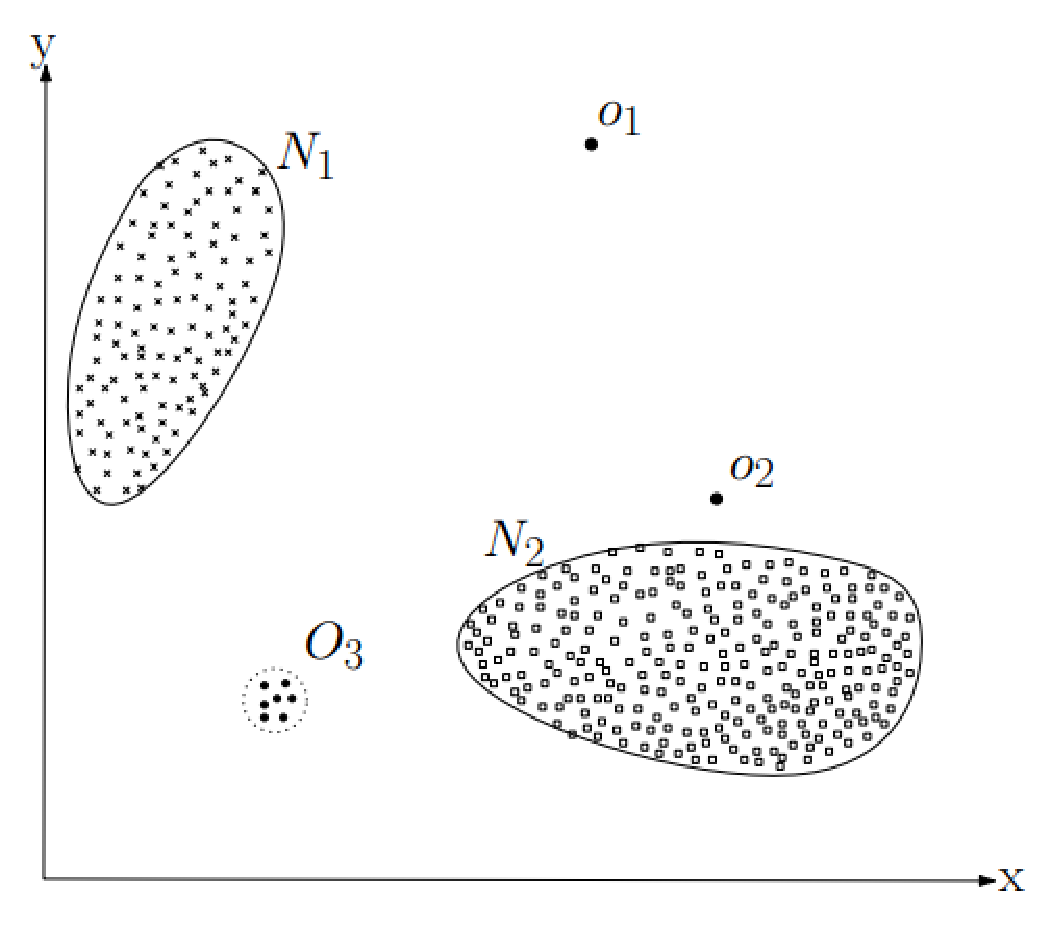
\includegraphics[width=0.5\textwidth]{2d-anomalies}
\caption[A simple example of anomalies in a 2-dimensional data set.]{A simple 
example of anomalies in a 2-dimensional data set \cite{Chandola:2007}.}
\label{fig:2d-anomalies}
\end{figure}

% CHALLENGES
\subsection{Challenges}
\label{sec:anomalyDetectionChallenges}
A straightforward anomaly detection approach, is to define a region representing
`normal' behaviour and declare any observation in the data which does not belong
to this normal region as an anomaly. But several factors make this apparently 
simple approach very challenging:

\begin{itemize}
\item Defining a normal region which encompasses every possible normal behaviour 
is very difficult. In addition, the boundary between normal and anomalous 
behaviour is often not precise. Thus an anomalous observation which lies close
to the boundary can actually be normal, and vice-versa.
\item When anomalies are the result of malicious actions, the malicious 
adversaries often adapt themselves to make the anomalous observations appear 
like normal, thereby making the task of defining normal behavior more difficult.
\item In many domains normal behavior keeps evolving and a current notion of
normal behavior might not be sufficiently representative in the future.
\item The exact notion of an anomaly is different for different application 
domains. For example, in the medical domain a small deviation from normal (for
example, fluctuations in body temperature) might be an anomaly, while similar 
deviation in the stock market domain (for example, fluctuations in the value of 
a stock) might be considered as normal. Thus applying a technique developed in 
one domain to another is not straightforward.
\item Availability of labeled data for training/validation of models used by 
anomaly detection techniques is usually a major issue.
\item Often the data contains noise which tends to be similar to the actual 
anomalies and hence is difficult to distinguish and remove.
\end{itemize}

Due to the above challenges, the anomaly detection problem, in its most general
form, is not easy to solve. In fact, most of the existing anomaly detection 
techniques solve a specific formulation of the problem. The formulation is 
induced by various factors such as nature of the data, availability of labeled 
data, type of anomalies to be detected, etc. Often, these factors are determined
by the application domain in which the anomalies need to be detected. 
Researchers have adopted concepts from diverse disciplines such as statistics, 
machine learning, data mining, information theory, spectral theory, and have 
applied them to specific problem formulations.

Researchers have adopted concepts from diverse disciplines such as statistics, 
data mining, statistics, information theory and spectral theory in order to gain
an increased understanding of anomalies \cite{Chandola:2007}.

% SIMILAR PROBLEMS
\subsection{Similar problems}
\label{sec:similarProblems}
Anomaly detection is an intentionally broad specifier for a class of 
more-specific statisctical challenges. For example, whilst being distinct from, 
anomaly detection is a similar problem (in terms of complexity and approach) to 
that of \emph{noise removal} and \emph{noise accomodation}, both of which are 
aimed at removing the effects of unwanted \emph{noise} in the data. Noise can be
defined as any data which is not of specific interest to the analyst, but in its
presence hinders data analysis techniques \cite{Chandola:2007}. It is often 
critical to data analysis to remove or mitigate the effects that noise has to 
the properties of the host data set.

In contrast, the problem of \emph{novelty detection} can often be impeded by 
techniques that attempt to remove anomalous data from a data set. \emph{Novelty 
detection} is process of discovering emerging patterns in a data set, to provide
an indication of the future state of a system. The distinction between novel
pattern and anomalies is that novel patterns are incorporated into the data 
model after detection \cite{Chandola:2007}.

% CLASSIFICATION
\subsection{Classification}
\label{sec:anomalyClassification}
In general, two different kinds of outliers exist: global outliers and local 
outliers. Global outliers are distinct with respect to the whole data set, while
local outliers are distinct with respect to data points in their local 
neighbourhood \cite{Vries:2011}. The task of global outlier detection has 
undergone much research \citeneeded{}, but this has not been the case for local 
outlier detection. In the paper \citetitle{Vries:2011}, \citeauthor{Vries:2011} 
optimise the use of local outlier factor (LOF) for large and high-dimensional 
data and propose projection-indexed nearest-neighbours (PINN) --- a novel 
technique that exploits extended nearest-neighbour sets in a reduced-dimensional
space --- to create an accurate approximation for k-nearest-neighbour distances, 
which is used as the core density measurement within LOF \cite{Vries:2011}.

\subsection{Types of anomalies}
\label{sec:typesOfAnomalies}
Anomalies can be classified into three categories \cite{Chandola:2007}:

\begin{description}
\item[Point anomaly] If an individual data instance can be considered as 
anomalous with respect to the rest of data, then the instance is termed as a 
point anomaly. This is the simplest type of anomaly. Referring to 
\hyperref[fig:2d-anomalies]{Figure~\ref{fig:2d-anomalies}}, points $o_{1}$ and 
$o_{2}$, as well as all points in region $O_{3}$ lie outside the boundary of the
normal regions, and are hence point anomalies.

\item[Contextual anomalies] If a data instance is anomalous in a certain 
context, but not otherwise, then it is termed a contextual anomaly. The notion 
of a context is induced by the structure in the data set and has to be specified
as part of the problem formulation.

\begin{figure}
\centering
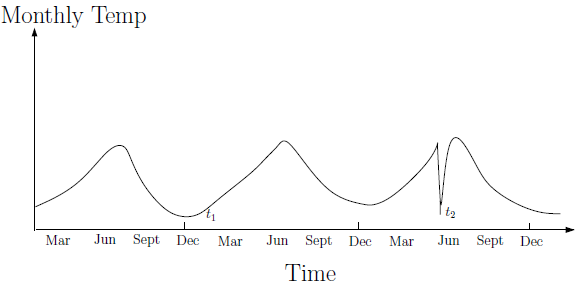
\includegraphics[width=0.5\textwidth]{contextual-anomalies}
\caption[Contextual anomaly $t_{2}$ in a temperature time series.]{Contextual 
anomaly $t_{2}$ in a temperature time series. Note that the temperature at time 
$t_{1}$ is same as that at time $t_{2}$ but occurs in a different context and 
hence is not considered as an anomaly \cite{Chandola:2007}.}
\label{fig:contextual-anomalies}
\end{figure}

Contextual anomalies have been most commonly explored in time-series data and 
spatial data. \hyperref[fig:contextual-anomalies]
{Figure~\ref{fig:contextual-anomalies}} shows one such example for a temperature
time series which shows the monthly temperature of an area over last few years. 
A temperature of $35\degree F$ might be normal during the winter (at time 
$t_{1}$) at that place, but the same value during summer (at time $t_{2}$) would
be an anomaly.

\item[Collective anomalies] If a collection of related data instances is 
anomalous with respect to the entire data set, it is termed as a collective 
anomaly. The individual data instances in a collective anomaly may not be 
anomalies by themselves, but their occurrence together as a collection is 
anomalous. \hyperref[fig:collective-anomalies]
{Figure~\ref{fig:collective-anomalies}} illustrates an example which shows a 
human electrocardiogram output. The highlighted region denotes an anomaly 
because the same low value exists for an abnormally long time. Note that that 
low value by itself is not an anomaly.

\begin{figure}
\centering
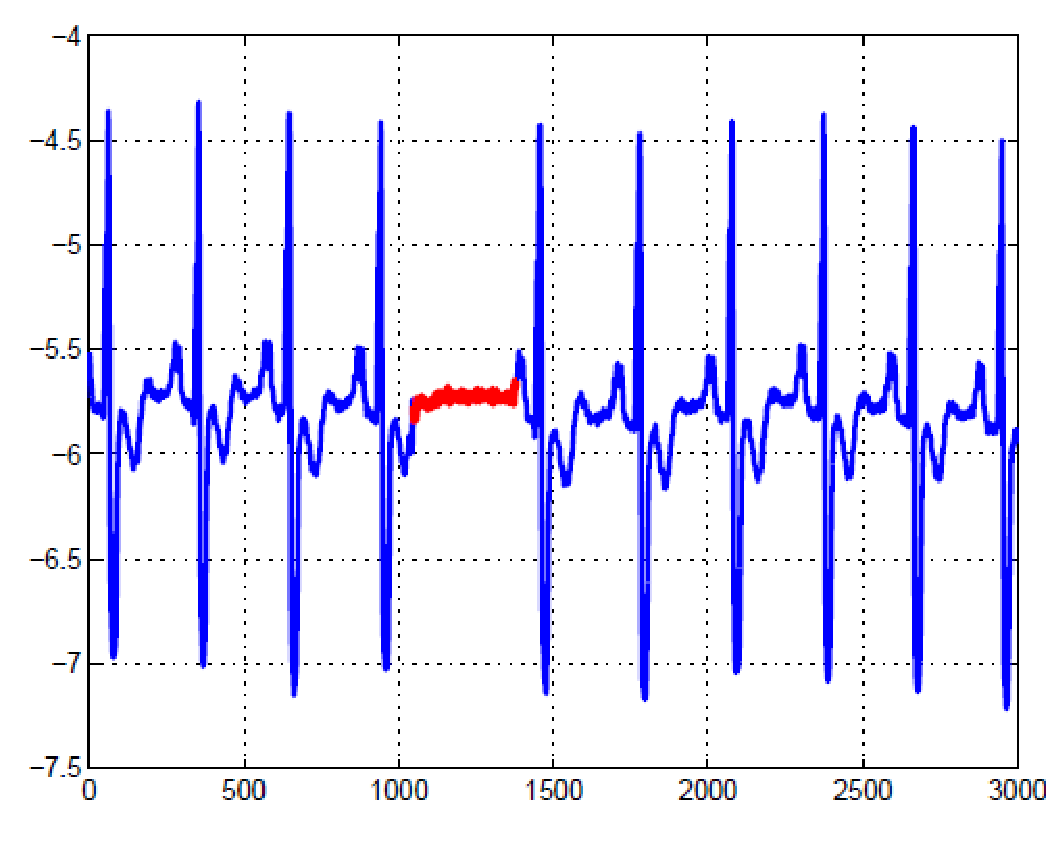
\includegraphics[width=0.5\textwidth]{collective-anomalies}
\caption[Collective anomaly corresponding to an \emph{Atrial Premature 
Contraction} in an human electrocardiogram output.]{Collective anomaly 
corresponding to an \emph{Atrial Premature Contraction} in an human 
electrocardiogram output \cite{Goldberger:2000}.}
\label{fig:collective-anomalies}
\end{figure}

\end{description}

% APPROACHES
\subsection{Approaches}

\begin{description}
\item[Classical] A point is declared to be an outlier if its distance from the 
mean is sufficiently large.
\item[Principal Component Analysis] An outlier is usually declared if the point 
is sufficiently far away from the subspace spanned by the eigenvectors 
corresponding to the highest eigenvalues.
\item[Distance based] A point can be declared to be an outlier if its distance 
to its kth nearest-neighbour is sufficiently large.
\item[Statistical based] Statistical methods are often model-based and assume 
that the data should follow some distribution. With knowledge of the 
distribution, data point are evaluated by their fitness to the assumed 
distribution. If the probability of a data instance is less than a certain 
threshold, then that data point is considered an anomaly.
\end{description}

Although distance is an effective non-parametric approach to detecting outliers,
the drawback is the amount of computation time required. Straightforward 
algorithms, such as those based on nested loops, typically require $O(N^{2})$
distance computations. This quadratic scaling means that it will be very 
difficult to mine outliers as we tackle increasingly larger data sets. This is a 
major problem for many real databases where there are often millions of records 
\cite{Bay:2003}.

\subsubsection{Distance based}
In this approach, one looks at the local neighborhood of points for an example 
typically defined by the $k$ nearest examples (also known as neighbours). If the
neighbouring points are relatively close, then the example is considered normal;
if the neighbouring points are far away, then the example is considered unusual.
The advantages of distance-based outliers are that no explicit distribution 
needs to be defined to determine unusualness, and that it can be applied to any 
feature space for which we can define a distance measure \cite{Bay:2003}.

Researchers have tried a variety of approaches to find these outliers 
efficiently. The simplest are those using nested loops \cite{Bay:2003}. In the 
basic version one compares each example with every other example to determine 
its $k$ nearest neighbors. Given the neighbors for each example in the data set,
simply select the top $n$ candidates according to the outlier definition. This 
approach has quadratic complexity as we must make all pairwise distance 
computations between examples.

Another method for finding outliers is to use a spatial indexing structure such 
as a KD-tree, R-tree, or X-tree to find the nearest neighbors of each candidate 
point. One queries the index structure for the closest $k$ points to each 
example, and as before one simply selects the top candidates according to the 
outlier definition. For low-dimensional data sets this approach can work 
extremely well and potentially scales as $O(N \log N)$ if the index tree can
find an example's nearest neighbors in $\log N$ time. However, index structures 
break down as the dimensionality increases \cite{Bay:2003}.

\subsubsection{Statistical based}
A common distribution considered when modelling data is the `Normal' 
distribution. Using this model, the probability that a data instance lies within
$k$ standard deviations $\sigma$ from the mean $\mu$ is the area between 
$\mu - k\sigma$ and $\mu + k\sigma$.

% LOCAL OUTLIER FACTOR
\subsection{Local Outlier Factor}
\label{sec:localOutlierFactor}
`Local Outlier Factor' is a formula that captures the degree to which a data 
point is an outlier with respect to its local neighbourhood. In this context,
`local' means that the determination of the data points does not depend on 
knowledge of the global distribution of the data set.

%%%%%%%%%%%%%%%%%%%%%%%%%%%%%%%%%%%%%%%%%%%%%%%%%
% VECTORS AND MATRICES
%%%%%%%%%%%%%%%%%%%%%%%%%%%%%%%%%%%%%%%%%%%%%%%%%
\section{Vectors and Matrices}
\label{sec:vectorsAndMatrices}

% EIGENVECTORS AND EIGENVALUES
\subsection{Eigenvectors and Eigenvalues}
\label{sec:eigenvectorsAndEigenvalues}
This section will briefly recall some basic definitions of eigenvectors and
eigenvalues, as well as some of their basic properties.

A vector $\mathbf{v}$ is an eigenvector of a matrix $M$ of eigenvalue $\lambda$ 
if:
\begin{equation}
M\mathbf{v} = \lambda\textbf{v}
\end{equation}

If $\mathbf{v_{1}}$ is an eigenvector of $M$ of eigenvalue $\lambda_{1}$, 
$\mathbf{v_{2}}$ is an eigenvector of $M$ of eigenvalue $\lambda_{2} \neq 
\lambda_{1}$, and $M$ is symmetric, then $\mathbf{v_{1}}$ is orthogonal to 
$\mathbf{v_{2}}$.

For a symmetric matrix $M$, the multiplicity of an eigenvalue $\lambda$ is the
dimension of the space of eigenvectors of eigenvalue $\lambda$. Also recall that
every $n{\times}n$ symmetric matrix has $n$ eigenvalues, counted with 
multiplicity. Thus, it has an orthonormal basis of eigenvectors, 
$\begin{Bmatrix} \mathbf{v_{1}} & \ldots & \mathbf{v_{n}} \end{Bmatrix}$ with
eigenvalues $\lambda_{1} \leq \lambda_{2} \leq \ldots \leq \lambda_{n}$ so that:
\begin{equation}
M\mathbf{v_{i}} = \lambda_{i}\mathbf{v_{i}} \quad \forall i
\end{equation}

If we let $V$ be the matrix whose $i$th column is $v_{i}$ and $\Lambda$ be the 
diagonal matrix whose $i$th diagonal is $\lambda_{i}$, we can write this more 
compactly as:
\begin{equation}
MV = V\Lambda
\end{equation}

Multiplying by $V^{T}$ on the right, we obtain the eigen-decomposition of $M$:
\begin{equation}
M = MVV^{T} = V{\Lambda}V^{T} = \sum_{i} \lambda_{i}\mathbf{v_{i}}\mathbf{v_{i}^{T}}
\end{equation}

% EIGEN DECOMPOSITION
\subsection{Eigen decomposition}
\label{sec:eigenDecomposition}
% TODO

% LAPLACIAN MATRICES
\subsection{Laplacian Matrices}
\label{sec:laplacianMatrices}
\nocite{Berkeley:1999}
\nocite{Pati:2011}
\nocite{Spielman:2006}
Recall that a weighted, undirected graph $G = (V,E,w)$ is essentially an 
undirected graph $G = (V,E)$ along with a function $w : E \rightarrow 
\Re^{+}$, where $\Re^{+}$ denotes the set of positive real numbers.

The adjacency matrix of a weighted graph $G$ is be denoted $A_{G}$, and is
given by:
\begin{equation}
A_{G}(i,j) := 
    \left\{
        \begin{array}{ll}
            \mathit{w}(i,j) &   \quad \text{if $(i,j) \in E$} \\
            0 &                 \quad \text{otherwise}
        \end{array}
    \right.
\end{equation}

The degree matrix of a weighted graph $G$, denoted $D_{G}$, is the diagonal 
matrix such that:
\begin{equation}
D_{G}(i,i) = \sum_{j} A_{G}(i,j)
\end{equation}

A Laplacian Matrix is a matrix representation of a graph, defined by the
equation:
\begin{equation}
L_{G} = D_{G} - A_{G}
\end{equation}

For a vector $\textbf{x} \in \Re^{V}$, the Laplacian quadratic form of $G$ is:
\begin{equation}
\label{eqn:laplacianQuadraticForm}
\textbf{x}^{T} L \textbf{x} = \sum_{(u,v) \in E} w_{u,v}(\textbf{x}(u) - \textbf{x}(v))^2
\end{equation}

From \hyperref[eqn:laplacianQuadraticForm]
{Equation~\ref{eqn:laplacianQuadraticForm}}, it can be seen that $L$ provides a 
measure of the smoothness of $\textbf{x}$ over the edges in $G$. The more 
$\textbf{x}$ jumps over an edge, the larger the quadratic form becomes.

It is often more convenient to consider the normalized Laplacian of a graph 
instead of the Laplacian \cite{Spielman:2010}. The normalized Laplacian is given
by $D^{-1/2}LD^{-1/2}$ and is more closely related to the behaviour of random 
walks.

Now, let $G_{1,2}$ be a graph on two vertices with a single edge of weight $1$.
\begin{equation}
L_{G_{1,2}} :=
    \begin{bmatrix}
        1 & -1 \\
        -1 & 1
    \end{bmatrix}
\end{equation}

For the graph with $n$ vertices and just one edge between vertices $u$ and $v$, 
we can define the Laplacian Matrix similarly. For concreteness, I'll call this
graph $G_{u,v}$. It's Laplacian Matrix is the $n{\times}n$ matrix whose only 
non-zero entries are in the intersections of rows and columns $u$ and $v$. The 
$2{\times}2$ matrix at the intersections of these rows and columns is, of 
course:
\begin{equation}
    \begin{bmatrix}
        1 & -1 \\
        -1 & 1
    \end{bmatrix}
\end{equation}

For a weighted graph $G = (V,E,w)$, we define:
\begin{equation}
L_{G} := \sum_{(u,v) \in E} w(u,v)L_{G_{u,v}}
\end{equation}

\subsubsection{Properties}
Laplacian matrices of graphs are symmetric, have zero row-sums, and have nonpositive
off-diagonal entries. We call any matrix that satisfies these properties a
Laplacian matrix, as there always exists some graph for which it is the Laplacian \cite{Spielman:2010}.

For a graph $G$ and its Laplacian Matrix $L$ with eigenvalues $\lambda_{0} < 
\lambda_{1} < \ldots < \lambda_{n-1}$:

\begin{itemize}
\item $L$ is a symmetric matrix. This means the eigenvalues of $L$ are real, and
its eigenvectors are real and orthogonal.
\item $L$ is always positive-semidefinite ($\forall i, \lambda_{i} \geq 0; 
\lambda_{0} = 0$).
\item Let $G = (V,E)$ be a graph, and let $0 = \lambda_{1} \leq \lambda_{2}
\leq \ldots \leq \lambda_{n}$ be the eigenvalues of its Laplacian Matrix. Then, 
$\lambda_{2} > 0$ if and only if $G$ is connected.
\item The number of times $0$ appears as an eigenvalue in the Laplacian Matrix 
is the number of connected components in the graph.
\item $\lambda_{0}$ is always $0$ because every Laplacian Matrix has an 
eigenvector of $\begin{bmatrix} 1 & 1 & \ldots & 1 \end{bmatrix}$ that, for each
row, adds the corresponding node's degree to a ``-1'' for each neighbour, 
thereby producing zero by definition.
\item The smallest non-zero eigenvalue of $L$ is called the spectral gap.
\item If we arbitrarily assign an orientation to the edges in $G$ and label each
edge, then we can define the vertex edge incidence matrix $Q$ by:
\begin{equation}
Q_{ij} := 
    \left\{
        \begin{array}{ll}
            1 &     \quad \text{if $e_{j}$ starts from $i$} \\
            -1 &    \quad \text{if $e_{j}$ ends at $i$} \\
            0 &     \quad \text{otherwise}
        \end{array}
    \right.
\end{equation}
Then the Laplacian Matrix $L$ satisfies $L = Q^{T}Q$, regardless of the 
orientation of the edges.
\item The second smallest eigenvalue of $L$ ($\lambda_{2}$) is the algebraic 
connectivity of $G$. $\lambda_{2} > 0$ if and only if $G$ is connected.
\end{itemize}

\subsubsection{Applications}
An interesting application of Laplacian matrices is that of modelling electrical
flow in a network resistors. In this model, the vertices of the graph correspond
to points at which current can be added to or removed from the circuit. Edges in
the graph correspond to resistors, with the edge weight equal to the conductance
of the electrical resistor.

If $\textbf{p} \in \Re^{V}$ denotes the vector of potentials and 
$\textbf{i}_{ext} \in \Re^{V}$ the vectors of currents entering and leaving 
vertices, then these satisfy the relation:
\begin{equation}
L\textbf{p} = \textbf{i}_{ext}
\end{equation}

This equation can be exploited to o compute the effective resistance between 
pairs of vertices \cite{Spielman:2010}. The effective resistance between 
vertices $u$ and $v$ is the difference in potential one must impose between $u$ 
and $v$ to flow one unit of current from $u$ to $v$. To measure this, we compute
the vector $\textbf{p}$ for which $L\textbf{p} = \textbf{i}_{ext}$, where:
\begin{equation}
\textbf{i}_{ext}(x) =
	\left\{
        \begin{array}{ll}
            1 &   	\quad \text{for $x=u$} \\
            -1 & 	\quad \text{for $x=v$} \\
            0 &		\quad \text{otherwise}
        \end{array}
    \right.
\end{equation}

We then measure the difference between $\textbf{p}(u)$ and $\textbf{p}$(v).

%%%%%%%%%%%%%%%%%%%%%%%%%%%%%%%%%%%%%%%%%%%%%%%%%
% COMMUTE TIME
%%%%%%%%%%%%%%%%%%%%%%%%%%%%%%%%%%%%%%%%%%%%%%%%%
\section{Commute Time}
\label{sec:commuteTime}

% INTRODUCTION
\subsection{Introduction}
\label{sec:commuteTimeIntroduction}
Commute time is a robust distance metric derived from a random walk on graphs 
\cite{Khoa:2012}. In \citetitle{Khoa:2012}, \citeauthor{Khoa:2012} demonstrated 
how commute time can be used as a distance measure for data mining tasks such as
anomaly detection and clustering. A prohibitive limitation of this technique is 
that the calculation of commute time involves the eigen decomposition of the 
graph Laplacian, making it impractical for large graphs.

A major advantage of using commute time as a distance metric for outlier 
detection is that it effectively captures not only the distances between data 
points but also the density of the data \citeneeded{}. This property results in 
a distance metric that can be effectively used to capture global, local and 
group anomalies.

The commute time between two nodes $i$ and $j$ in a graph is the number of steps
that a random walk, starting from $i$ will take to visit $j$ and then come back 
to $i$ for the first time. The fact that the commute time is averaged over all 
paths (and not just the shortest path) makes it more robust to data 
perturbations and it can also capture graph density \cite{Khoa:2012}. Since it 
is a measure which can capture the geometrical structure of the data and is 
robust to noise, commute time can be applied in methods where Euclidean or other
distances are used and thus the limitations of these metrics can be avoided.

% LIMITATIONS
\subsection{Limitations}
\label{sec:commuteTime:limitations}
The computation of commute time requires the eigen decomposition (see 
\hyperref[sec:eigenDecomposition] {Section~\ref{sec:eigenDecomposition}}) of the
graph Laplacian matrix (see \hyperref[sec:laplacianMatrices] 
{Section~\ref{sec:laplacianMatrices}}), a computation which takes $O(n^{3})$ 
time and thus is not practical for large graphs \citeneeded{}. Methods to 
approximate the commute time to reduce the computational time are required in 
order to efficiently use commute time in large datasets.

% ANOMALY DETECTION USING COMMUTE TIME
\subsection{Anomaly Detection Using Commute Time}
\label{sec:anomalyDetectionUsingCommuteTime}
% TODO

%%%%%%%%%%%%%%%%%%%%%%%%%%%%%%%%%%%%%%%%%%%%%%%%%
% DISTANCE METRICS
%%%%%%%%%%%%%%%%%%%%%%%%%%%%%%%%%%%%%%%%%%%%%%%%%
\section{Distance metrics}
\label{sec:distanceMetrics}
Distance is a quantitative description of how far apart two objects are. 
Mathematically, a distance or metric is a function describing how close or far 
away data points in some space are from each other \cite{Khoa:2012}.

% EUCLIDEAN DISTANCE
\subsection{Euclidean distance}
\label{sec:euclideanDistance}
An Euclidean distance between two data points in a space is the norm of the 
difference between two vectors corresponding to these data points 
\cite{Khoa:2012}. Euclidean distance is extremely sensitive to the scale of the 
features involved. When dealing with features of vastly different scales, the 
effects of the larger feature dominant over the smaller feature in terms of the 
Euclidean distance. This problem is usually solved by normalizing the data 
values. Another issue, however, with Euclidean distance is that it is unable to 
take into account any correlation between data features.

% MAHALANOBIS DISTANCE
\subsection{Mahalanobis distance}
\label{sec:mahalanobisDistance}
Mahalanobis distance is a distance measure that considers the covariance between
data features. Mahalanobis distance, however, is extremely sensitive to 
anomalies as anomalies affect both the mean and the covariance of the data.

% GRAPH GEODESIC DISTANCE
\subsection{Graph geodesic distance}
\label{sec:graphGeodesicDistance}
% TODO

%%%%%%%%%%%%%%%%%%%%%%%%%%%%%%%%%%%%%%%%%%%%%%%%%
% MARKOV CHAINS
%%%%%%%%%%%%%%%%%%%%%%%%%%%%%%%%%%%%%%%%%%%%%%%%%
\section{Markov chains}
\label{sec:markovChains}
A `Markov chain' is a chance process in which the outcome of a given experiment 
can affect the outcome of the next experiment \cite{Grinstead:1997}. For a 
Markov chain, we have a set of states $S = \left\{ s_{1}, s_{2}, \ldots, s_{r} 
\right\}$ with a process starting in one of the states and moving from state 
$s_{i}$ to $s_{j}$ with a probability $p_{ij}$ not dependent upon which states 
the chain was in before the current state. The probabilities $p_{ij}$ are called
\emph{transition probabilities}, and the complete matrix $\mathbf{P}$ of 
probabilities is known as the \emph{transition matrix}.

The probability that, given the chain is in state $i$ now, it will be in state 
$j$ in two steps is denoted by $p_{ij}^{(2)}$. In general, if a Markov chain has 
$r$ states, then:

\begin{equation}
p_{ij}^{(2)} = \sum_{k=1}^{r} p_{ik}p{kj}
\end{equation}

%%%%%%%%%%%%%%%%%%%%%%%%%%%%%%%%%%%%%%%%%%%%%%%%%
% RANDOM PROJECTIONS
%%%%%%%%%%%%%%%%%%%%%%%%%%%%%%%%%%%%%%%%%%%%%%%%%
\section{Random projections}
\label{sec:randomProjections}
% TODO

%%%%%%%%%%%%%%%%%%%%%%%%%%%%%%%%%%%%%%%%%%%%%%%%%
% RANDOM WALKS ON GRAPHS
%%%%%%%%%%%%%%%%%%%%%%%%%%%%%%%%%%%%%%%%%%%%%%%%%
\section{Random walks on graphs}
\label{sec:randomWalks}

Assume we are given a connected undirected and weighted graph $G = (V,E,W)$ with
edge weights $(w_{ij})_{i,j \in V} >= 0$ be the graph adjacency matrix. A degree
of a node $i$ is $d_{i} = \sum_{j \in N(i)} w_{ij}$ where $N(i)$ is a set of 
neighbours of node $i$. All nodes nonadjacent to $i$ are assumed to have a 
weight of $w_{ij} = 0$.

A random walk is a sequence of nodes on a graph visited by a random walker: 
starting from a node, the random walker moves to one of its neighbours with some
probability. Then from that node, it proceeds to one of its own neighbours with 
some probability, and so on \cite{Khoa:2012}. The random walk is a finite Markov
chain that is time-reversible, which means the reverse Markov chain has the same
transition probability matrix as the original Markov chain \cite{Lovasz:1996}.

The probability that a random walker selects a particular node from is 
neighbours is determined by the edge weights of the graph. The larger the weight
${w_ij}$ of the edge connecting nodes $i$ and $j$, the more often the random 
walker travels through that edge.

%%%%%%%%%%%%%%%%%%%%%%%%%%%%%%%%%%%%%%%%%%%%%%%%%
% NEAREST NEIGHBOUR ALGORITHMS
%%%%%%%%%%%%%%%%%%%%%%%%%%%%%%%%%%%%%%%%%%%%%%%%%
\section{Nearest Neighbour Algorithms}
\label{sec:nearestNeighbourAlgorithms}
% TODO

%%%%%%%%%%%%%%%%%%%%%%%%%%%%%%%%%%%%%%%%%%%%%%%%%
% SOLVERS
%%%%%%%%%%%%%%%%%%%%%%%%%%%%%%%%%%%%%%%%%%%%%%%%%
\section{Solvers}
\label{sec:solvers}

% SPIELMAN-TENG SOLVER
\subsection{Spielman-Teng Solver}
\label{sec:spielmanTengSolver}
\nocite{Spielman:2006}
Spielman and Teng presented a randomised algorithm that, on input a symmetric, 
weakly diagonally dominant $n{\times}x$ matrix $A$ with $m$ non-zero entries and
an $n$-vector $\mathbf{b}$, produces an $\tilde{\mathbf{x}}$ such that 
$\begin{Vmatrix} \tilde{\textbf{x}} - A^{\dagger}\textbf{b} \end{Vmatrix}_{A} 
\leq \epsilon \begin{Vmatrix} A^{\dagger}\mathbf{b} \end{Vmatrix}_{A}$ in 
expected time:
\begin{equation}
m \log^{O(1)} n \log (1/\epsilon)
\end{equation}


%%%%%%%%%%%%%%%%%%%%%%%%%%%%%%%%%%%%%%%%%%%%%%%%%
% CHAPTER 03: Reconfigurable Computing
%%%%%%%%%%%%%%%%%%%%%%%%%%%%%%%%%%%%%%%%%%%%%%%%%
\chapter{Reconfigurable Computing}
\label{ch:reconfigurableComputing}

\section{Introduction}
\label{sec:rcIntroduction}
In the computer and electronics world, computations are performed either in 
hardware or in software. Computer hardware provides highly optimized resources
for quickly performing critical tasks, but is permanently configured to a 
single task or application. Computer software offers a flexible approach, but is
orders of magnitude worse than a hardware implementation in terms of 
performance, silicon area efficiency and power consumption.

FPGAs are devices that combine the advantages of hardware implementations with 
the flexibility of software implementations. The computations are programmed 
into the silicon chip such that an FPGA system can be programmed and 
reprogrammed many times. The utility of FPGAs does, however, come at a price. 
Whilst, compared to a microprocessor, FPGAs are typically several orders of 
magnitude faster and more power efficient, the task of creating efficient 
programs for these devices is difficult.

Typically, FPGAs are useful only for operations that process large streams of 
data, such as signal processing, networking, and the like. Compared to 
integrated circuit, they may be 5 to 25 times worse in terms of area, delay, and
performance \cite{Hauck:2007}. However, while an integrated circuit design may 
take months to years to develop and have a multimillion-dollar price tag, an 
FPGA design might only take days to create and cost tens to hundreds of dollars.

\section{Field-Programmable Gate Array (FPGA)}
\label{sec:FPGA}


%%%%%%%%%%%%%%%%%%%%%%%%%%%%%%%%%%%%%%%%%%%%%%%%%
% CHAPTER 04: Design
%%%%%%%%%%%%%%%%%%%%%%%%%%%%%%%%%%%%%%%%%%%%%%%%%
\chapter{Design}
\label{ch:design}

\section{Introduction}
\label{sec:designIntroduction}

% ALGORITHM PROFILING
\section{Algorithm Profiling}
\label{sec:algorithmProfiling}
In order to choose which step of the algorithm would be best suited for 
implementation on FPGA hardware, it was first necessary to first profile the 
execution of the algorithm using various test cases. This task was performed 
using \emph{MATLAB}, using code supplied by \citeauthor{Khoa:2012} that was used
to test and verify the conclusions of \citetitle{Khoa:2012}. Using 
\emph{MATLAB}'s \verb+profile+ command, I was able to analyse the algorithm and 
make an assessment of the running time of the algorithm.

% PERFORMANCE BOTTLENECK
\subsection{Performance Bottleneck}
\label{sec:algorithmPerformanceBottleneck}
From observations of the MATLAB execution profile.


%%%%%%%%%%%%%%%%%%%%%%%%%%%%%%%%%%%%%%%%%%%%%%%%%
% CHAPTER 05: Implementation
%%%%%%%%%%%%%%%%%%%%%%%%%%%%%%%%%%%%%%%%%%%%%%%%%
\chapter{Implementation}
\label{ch:implementation}

%%%%%%%%%%%%%%%%%%%%%%%%%%%%%%%%%%%%%%%%%%%%%%%%%
% CHAPTER 06: Results
%%%%%%%%%%%%%%%%%%%%%%%%%%%%%%%%%%%%%%%%%%%%%%%%%
\chapter{Results}
\label{ch:results}

%%%%%%%%%%%%%%%%%%%%%%%%%%%%%%%%%%%%%%%%%%%%%%%%%
% CHAPTER 07: Conclusions
%%%%%%%%%%%%%%%%%%%%%%%%%%%%%%%%%%%%%%%%%%%%%%%%%
\chapter{Conclusions}
\label{ch:conclusions}

%%%%%%%%%%%%%%%%%%%%%%%%%%%%%%%%%%%%%%%%%%%%%%%%%
% Appendix
%%%%%%%%%%%%%%%%%%%%%%%%%%%%%%%%%%%%%%%%%%%%%%%%%
\appendix

%%%%%%%%%%%%%%%%%%%%%%%%%%%%%%%%%%%%%%%%%%%%%%%%%
% APPENDIX 01: Computer specifications
%%%%%%%%%%%%%%%%%%%%%%%%%%%%%%%%%%%%%%%%%%%%%%%%%
\chapter{Computer specifications}
\label{apdx:computerSpecifications}
All test results contained in this thesis were performed on a server with the 
following specifications. The following specifications were obtained using the
\doubleQuote{Hardware Lister} (\verb+lshw+) tool.

\begin{table}
    \centering
    \begin{tabular}{|+>{\bfseries}l|^l|}
        \tableHeader{Item & Specification}
        CPU &\\
        Product & Intel(R) Core(TM) i5 CPU M 540 @ 2.53GHz\\
        Capacity & 1199MHz\\
        Width & 64 bits\\
        Clock & 133MHz\\
        Cores & 2\\
        L1 cache & 32KiB (asynchronous internal write-through data)\\
        L2 cache & 256KiB (burst internal write-through unified)\\
        L3 cache & 8MiB (burst internal write-back)\\[1em]
        
        Memory &\\
        Description & SODIMM DDR3 Synchronous 1066 MHz\\
        Size & 4GiB\\
        Width & 64 bits\\
        Clock & 1066MHz\\\hline
    \end{tabular}
    \caption{Hardware specifications}
\end{table}

\begin{table}
    \centering
    \begin{tabular}{|+>{\bfseries}l|^l|}
        \tableHeader{Item & Specification}
        gcc & gcc (Ubuntu/Linaro 4.6.1-9ubuntu3) 4.6.1\\
        ld & GNU ld (GNU Binutils for Ubuntu) 2.21.53.20110810\\
        MATLAB & \\
        mex & \\\hline
    \end{tabular}
    \caption{Software specifications}
\end{table}

\begin{table}
    \centering
    \begin{tabular}{|+>{\bfseries}l|^l|}
        \tableHeader{Item & Specification}
        Operating System & Ubuntu 11.10\\
        Platform & x86\_64\\
        Kernel version & 3.0.0-17-generic\\\hline
    \end{tabular}
    \caption{Operating System specifications}
\end{table}


%%%%%%%%%%%%%%%%%%%%%%%%%%%%%%%%%%%%%%%%%%%%%%%%%
% APPENDIX 02: MATLAB code
%%%%%%%%%%%%%%%%%%%%%%%%%%%%%%%%%%%%%%%%%%%%%%%%%
\chapter{MATLAB Code}
\label{apdx:matlabCode}
\lstloadlanguages{Matlab}
\lstset{language=Matlab}
\begin{lstlisting}
% Find the top N outliers by comparing average distances
% to the k nearest neighbours with pruning technique.
function[O,OF]=TopN_Outlier_Pruning_Block(X,k,N,block_size)
	n = size(X,1);
	OF = zeros(1,N);
	O = OF;

	c = 0;
	count = 0;
	while (n-count > 0)
		B = zeros(1,block_size);
		B = (count+1 : count+block_size);
		count = count+block_size;

		if count <= n
			sizeB = block_size;
		else
			sizeB = n-(count-block_size);
		end

		neighbours = zeros(sizeB,k);
		neighbours_dist = zeros(sizeB,k);
		score = zeros(1,sizeB);

		l = 1;
		for i = 1:n
			for j = 1:sizeB
				if i~=B(j) && B(j)~=0
					d=euclidean_dist_squared(X(i,:),X(B(j),:));

					if l>1 && l<=k+1 && neighbours(j,l-1)==0
						l=l-1;
					elseif l<k && neighbours(j,l)~=0
						l=l+1;
					end

					if l<=k
						neighbours(j,l)=i;
						neighbours_dist(j,l)=d;
						if l==k
							score(j)=mean(neighbours_dist(j,:),2);
						end
					else % l>k
						% find the farthest point
						[maxd,maxi]=max(neighbours_dist(j,:));

						% replace the farthest point
						if d<maxd
							neighbours(j,maxi)=i;
							neighbours_dist(j,maxi)=d;

							% update the score
							score(j)=(score(j)*k-maxd+d)/k;
							if score(j)<=0
								% avoid round off error
								score(j)=max(mean(neighbours_dist(j,:),2),0);
							end
						end
					end

					if l>=k && score(j)<c
						B(j)=0;
						%neighbours(j,:)=0;
						%neighbours_dist(j,:)=0;
						score(j)=0;
					end
				end
			end
			l=l+1;
		end

		% O=Top(B U O,N)
		BO=[B(1:sizeB) O];
		BOF=[score OF];
		[BOF,index]=sort(BOF,'descend');
		BO=BO(index);

		O=BO(1:N);
		OF=BOF(1:N);

		%c=weakest outlier
		c=OF(N);
	end
\end{lstlisting}


%%%%%%%%%%%%%%%%%%%%%%%%%%%%%%%%%%%%%%%%%%%%%%%%%
% APPENDIX 03: C code
%%%%%%%%%%%%%%%%%%%%%%%%%%%%%%%%%%%%%%%%%%%%%%%%%
\chapter{C Code}
\label{apdx:cCode}
\lstloadlanguages{C}
\lstset{language=C}
\begin{lstlisting}
/* Includes */
#include <float.h> /* for DBL_MAX */
#include <string.h> /* for memset, memcpy */
#include "macros.h"
#include "top_n_outlier_pruning_block.h"

/* Check compatibility of defined macros. */
#if (defined(UNSORTED_INSERT) && defined(SORTED_INSERT)) || (!defined(UNSORTED_INSERT) && !defined(SORTED_INSERT))
	#error "Exactly one of UNSORTED_INSERT and SORTED_INSERT should be defined."
#endif /* #if defined(UNSORTED_INSERT) && defined(SORTED_INSERT) */

#if !defined(DEBUG) && defined(STATS)
	#error "STATS should only be defined in DEBUG mode."
#endif /* #if !defined(DEBUG) && defined(STATS) */

/* Forward declarations */
static inline double_t distance_squared(
	const double_t * const vector1, 
	const double_t * const vector2, 
	const size_t vector_dims
	);
static inline double_t insert(
	index_t * const outliers,
	double_t * const outlier_scores,
	const size_t k,
	uint_t * const found,
	const index_t new_outlier, 
	const double_t new_outlier_index
	);
static inline void best_outliers(
	index_t * const outliers,
	double_t * const outlier_scores,
	size_t * outliers_size,
	const size_t N,
	index_t * const current_block,
	double_t * const scores,
	const size_t block_size
	);
static inline void sort_vectors_descending(
	index_t *  const current_block,
	double_t * const scores,
	const size_t block_size
	);
static inline void merge(
	index_t * const global_outliers,
	double_t * const global_outlier_scores,
	const size_t global_outliers_size,
	const size_t N,
	index_t * const local_outliers,
	double_t * const local_outlier_scores,
	const size_t block_size,
	index_t * const new_outliers,
	double_t * const new_outlier_scores,
	size_t * new_outliers_size
	);

#ifdef STATS
static lint_t calls_counter = 0;
static uint_t num_pruned = 0;

void get_stats(lint_t * const counter, uint_t * const prune_count) {
	ASSERT_NOT_NULL(counter);
	ASSERT_NOT_NULL(prune_count);
	
	*counter = calls_counter;
	*prune_count = num_pruned;
}
#endif /* #ifdef STATS */

static inline double_t distance_squared(const double_t * const vector1, const double_t * const vector2, const size_t vector_dims) {
	ASSERT_NOT_NULL(vector1);
	ASSERT_NOT_NULL(vector2);
	ASSERT(vector_dims > 0);
	
#ifdef STATS
	const UNUSED lint_t old_calls_counter = calls_counter;
	calls_counter++;
	ASSERT(calls_counter > old_calls_counter);
#endif /* #ifdef STATS */
	
	double_t sum_of_squares = 0;
	
	uint_t dim;
	for (dim = 0; dim < vector_dims; dim++) {
		const double_t val = vector1[dim] - vector2[dim];
		const double_t val_squared = val * val;
		sum_of_squares += val_squared;
	}
	
	return sum_of_squares;
}

static inline double_t insert(index_t * const outliers,
							  double_t * const outlier_scores,
							  const size_t k,
							  uint_t * const found,
							  const index_t new_outlier, 
							  const double_t new_outlier_score) {
	/* Error checking. */
	ASSERT_NOT_NULL(outliers);
	ASSERT_NOT_NULL(outlier_scores);
	ASSERT(k > 0);
	ASSERT_NOT_NULL(found);
	ASSERT(*found <= k);
	ASSERT(new_outlier >= start_index);
	
	int_t	insert_index  = -1; /* the index at which the new outlier will be inserted */
	double_t removed_value = -1; /* the value that was removed from the outlier_scores array */
	
#if defined(SORTED_INSERT)
	/*
	 * Shuffle array elements from front to back. Elements greater than the new
	 * value will be right-shifted by one index in the array.
	 *
	 * Note that uninitialised values in the array will appear on the left. That
	 * is, if the array is incomplete (has a size n < N) then the data in the
	 * array is stored in the rightmost n indexes.
	 */
	
	if (*found < k) {
		/* Special handling required if the array is incomplete. */
		
		uint_t i;
		for (i = k - *found - 1; i < k; i++) {
			if (new_outlier_score > outlier_scores[i] || i == (k - *found - 1)) {
				/* Shuffle values down the array. */
				if (i != 0) {
					outliers[i-1] = outliers[i];
					outlier_scores[i-1] = outlier_scores[i];
				}
				insert_index  = i;
				removed_value = 0;
			} else {
				/* We have found the insertion point. */
				break;
			}
		}
	} else {
		int_t i;
		for (i = k-1; i >= 0; i--) {
			if (new_outlier_score < outlier_scores[i]) {
				if ((unsigned) i == k-1)
					/*
					 * The removed value is the value of the last element in the
					 * array.
					 */
					removed_value = outlier_scores[i];

				/* Shuffle values down the array. */
				if (i != 0) {
					outliers[i] = outliers[i-1];
					outlier_scores[i] = outlier_scores[i-1];
				}
				insert_index = i;
			} else {
				/* We have found the insertion point. */
				break;
			}
		}
	}
#elif defined(UNSORTED_INDEX)
	if (*found < k) {
		insert_index = *found + 1;
		removed_value = 0;
	} else {
		int_t max_index = -1;
		double_t max_value = DBL_MAX;
	
		int_t i;
		for (i = k-1; i >= 0; i--) {
			if (max_index <= 0 || outlier_scores[i] > max_value) {
				max_index = i;
				max_value = outlier_scores[i];
			}
		}
		
		if (new_outlier_score < max_value) {
			insert_index  = max_index;
			removed_value = max_value;
		}
	}
#endif /* #if defined(SORTED_INSERT) */
	
	/*
	 * Insert the new pair and increment the current_size of the array (if
	 * necessary).
	 */
	if (insert_index >= 0) {
		outliers[insert_index] = new_outlier;
		outlier_scores[insert_index] = new_outlier_score;
		
		if (*found < k)
			(*found)++;
	}
	
	return removed_value;
}

static inline void best_outliers(index_t * const outliers,
								 double_t * const outlier_scores,
								 size_t * outliers_size,
								 const size_t N,
								 index_t * const current_block,
								 double_t * const scores,
								 const size_t block_size) {
	/* Error checking. */
	ASSERT_NOT_NULL(outliers);
	ASSERT_NOT_NULL(outlier_scores);
	ASSERT_NOT_NULL(outliers_size);
	ASSERT(*outliers_size <= N);
	ASSERT(N > 0);
	ASSERT_NOT_NULL(current_block);
	ASSERT_NOT_NULL(scores);
	ASSERT(block_size > 0);
	
	/* Sort the (current_block, scores) vectors in descending order of value. */
	sort_vectors_descending(current_block, scores, block_size);
	
	/* Create two temporary vectors for the output of the "merge" function. */
	index_t  new_outliers[N];
	double_t new_outlier_scores[N];
	size_t   new_outliers_size = 0;
	
	memset(new_outliers, null_index, N * sizeof(index_t));
	memset(new_outlier_scores, 0, N * sizeof(double_t));
	
	/* Merge the two vectors. */
	merge(outliers, outlier_scores, *outliers_size, N, current_block, scores, block_size, new_outliers, new_outlier_scores, &new_outliers_size);
	
	/* Copy values from temporary vectors to real vectors. */
	memcpy(outliers, new_outliers, N * sizeof(index_t));
	memcpy(outlier_scores, new_outlier_scores, N * sizeof(double_t));
	*outliers_size = new_outliers_size;
}

static inline void sort_vectors_descending(index_t *  const current_block,
										   double_t * const scores,
										   const size_t block_size) {
	/* Error checking. */
	ASSERT_NOT_NULL(current_block);
	ASSERT_NOT_NULL(scores);
	ASSERT(block_size > 0);
	
	uint_t i;
	for (i = 0; i < block_size; i++) {
		int_t j;
		index_t  ind = current_block[i];
		double_t val = scores	   [i];
		for (j = i-1; j >= 0; j--) {
			if (scores[j] >= val)
				break;
			current_block[j+1] = current_block[j];
			scores	   [j+1] = scores	   [j];
		}
		current_block[j+1] = ind;
		scores	   [j+1] = val;
	}
}

static inline void merge(index_t * const global_outliers, double_t * const global_outlier_scores, const size_t global_outliers_size, const size_t N,
						 index_t * const local_outliers,  double_t * const local_outlier_scores,  const size_t block_size,
						 index_t * const new_outliers, double_t * const new_outlier_scores, size_t * new_outliers_size) {
	/* Error checking. */
	ASSERT_NOT_NULL(global_outliers);
	ASSERT_NOT_NULL(global_outlier_scores);
	ASSERT(global_outliers_size <= N);
	ASSERT(N > 0);
	ASSERT_NOT_NULL(local_outliers);
	ASSERT_NOT_NULL(local_outlier_scores);
	ASSERT(block_size > 0);
	ASSERT_NOT_NULL(new_outliers);
	ASSERT_NOT_NULL(new_outlier_scores);
	ASSERT_NOT_NULL(new_outliers_size);
	
	*new_outliers_size  = 0;
	uint_t iter = 0; /* iterator through output array */
	uint_t global = 0; /* iterator through global array */
	uint_t local = 0; /* iterator through local array */
	while (iter < N && (global < global_outliers_size || local < block_size)) {
		if (global >= global_outliers_size && local < block_size) {
			/* There are no remaining elements in the global arrays. */
			new_outliers[iter] = local_outliers[local];
			new_outlier_scores[iter] = local_outlier_scores[local];
			local ++;
			global++;
		} else if (global < global_outliers_size && local >= block_size) {
			/* There are no remaining elements in the local arrays. */
			new_outliers[iter] = global_outliers[global];
			new_outlier_scores[iter] = global_outlier_scores[global];
			local ++;
			global++;
		} else if (global >= global_outliers_size && local >= block_size) {
			/*
			 * There are no remaining elements in either the global or local 
			 * arrays.
			 */
			break;
		} else if (global_outlier_scores[global] >= local_outlier_scores[local]) {
			new_outliers[iter] = global_outliers[global];
			new_outlier_scores[iter] = global_outlier_scores[global];
			global++;
		} else if (global_outlier_scores[global] <= local_outlier_scores[local]) {
			new_outliers[iter] = local_outliers[local];
			new_outlier_scores[iter] = local_outlier_scores[local];
			local++;
		}
		
		iter++;
		(*new_outliers_size)++;
	}
}

void top_n_outlier_pruning_block(const double_t * const data,
								 const size_t num_vectors, const size_t vector_dims,
								 const size_t k, const size_t N, const UNUSED size_t default_block_size,
								 index_t * outliers, double_t * outlier_scores) {
	/* Error checking. */
	ASSERT_NOT_NULL(data);
	ASSERT(vector_dims > 0);
	ASSERT(k > 0);
	ASSERT(N > 0);
	ASSERT(default_block_size > 0);
	ASSERT_NOT_NULL(outliers);
	ASSERT_NOT_NULL(outlier_scores);
	
	/* Set output to zero. */
	memset(outliers, null_index, N * sizeof(index_t));
	memset(outlier_scores, 0, N * sizeof(double_t));
	
	double_t cutoff = 0; /* vectors with a score less than the cutoff will be removed from the block */
	size_t   outliers_found = 0; /* the number of initialised elements in the outliers array */
	
#ifndef NO_BLOCKING
	index_t  block_begin; /* the index of the first vector in the block currently being processed */
	size_t   block_size; /* block_size may be smaller than devfault_block_size if "num_vectors mod default_block_size != 0" */
	
	for (block_begin = 0; block_begin < num_vectors; block_begin += block_size) { /* while there are still blocks to process */
		block_size = MIN(block_begin + default_block_size, num_vectors) - block_begin; /* the number of vectors in the current block */
		ASSERT(block_size <= default_block_size);
		
		index_t current_block[block_size]; /* the indexes of the vectors in the current block */
		index_t neighbours[block_size][k]; /* the "k" nearest neighbours for each vector in the current block */
		double neighbours_dist[block_size][k]; /* the distance of the "k" nearest neighbours for each vector in the current block */
		double score[block_size]; /* the average distance to the "k" neighbours */
		uint_t found[block_size]; /* how many nearest neighbours we have found, for each vector in the block */
		
		/* Reset array contents */
		uint_t i;
		for (i = 0; i < block_size; i++) {
			if (i < block_size)
				current_block[i] = (index_t)((block_begin + i) + start_index);
			else
				current_block[i] = null_index;
		}
		memset(&neighbours, null_index, block_size * k * sizeof(index_t));
		memset(&neighbours_dist, 0, block_size * k * sizeof(double));
		memset(&score, 0, block_size * sizeof(double));
		memset(&found, 0, block_size * sizeof(uint_t));
		
		index_t vector1;
		for (vector1 = start_index; vector1 < num_vectors + start_index; vector1++) {
			uint_t block_index;
			for (block_index = 0; block_index < block_size; block_index++) {
				const index_t vector2 = current_block[block_index];
				
				if (vector1 != vector2 && vector2 >= start_index) {
					/*
					 * Calculate the square of the distance between the two
					 * vectors (indexed by "vector1" and "vector2")
					 */
					const double_t dist_squared = distance_squared(&data[(vector1-start_index) * vector_dims], &data[(vector2-start_index) * vector_dims], vector_dims);
					
					/*
					 * Insert the new (index, distance) pair into the neighbours
					 * array for the current vector.
					 */
					
					const double_t removed_distance = insert(neighbours[block_index], neighbours_dist[block_index], k, &found[block_index], vector1, dist_squared);
					
					/*
					 * Update the score (if the neighbours array was changed).
					 */
					if (removed_distance >= 0)
						score[block_index] = (double_t) ((score[block_index] * k - removed_distance + dist_squared) / k);
					
					/*
					 * If the score for this vector is less than the cutoff,
					 * then prune this vector from the block.
					 */
					if (found[block_index] >= k && score[block_index] < cutoff) {
						current_block[block_index] = null_index;
						score[block_index] = 0;
#ifdef STATS
						const UNUSED uint_t old_num_pruned = num_pruned;
						num_pruned++;
						ASSERT(num_pruned > old_num_pruned);
#endif /* #ifdef STATS */
					}
				}
			}
		}
		
		/* Keep track of the top "N" outliers. */
		best_outliers(outliers, outlier_scores, &outliers_found, N, current_block, score, block_size);
		
		/*
		 * Set "cutoff" to the score of the weakest outlier. There is no need to
		 * store an outlier in future iterations if its score is better than the
		 * cutoff.
		 */
		cutoff = outlier_scores[N-1];
	}
#else
	index_t vector1;
	for (vector1 = start_index; vector1 < num_vectors + start_index; vector1++) {
		index_t neighbours[k]; /* the "k" nearest neighbours for the current vector */
		double_t neighbours_dist[k]; /* the distance of the "k" nearest neighbours for the current vector */
		double_t score = 0; /* the average distance to the "k" neighbours */
		uint_t found = 0; /* how many nearest neighbours we have found */
		boolean removed = false; /* true if vector1 has been pruned */
		
		memset(neighbours, null_index, k * sizeof(index_t));
		memset(neighbours_dist, 0, k * sizeof(double_t));
		
		index_t vector2;
		for (vector2 = start_index; vector2 < num_vectors + start_index && !removed; vector2++) {
			if (vector1 != vector2) {
				/*
				 * Calculate the square of the distance between the two
				 * vectors (indexed by "vector1" and "vector2")
				 */
				const double_t dist_squared = distance_squared(&data[(vector1-start_index) * vector_dims], &data[(vector2-start_index) * vector_dims], vector_dims);
				
				/*
				 * Insert the new (index, distance) pair into the neighbours
				 * array for the current vector.
				 */
				const double_t removed_distance = insert(neighbours, neighbours_dist, k, &found, vector2, dist_squared);
				
				/* Update the score (if the neighbours array was changed). */
				if (removed_distance >= 0)
					score = (double_t) ((score * k - removed_distance + dist_squared) / k);
				
				/*
				 * If the score for this vector is less than the cutoff,
				 * then prune this vector from the block.
				 */
				if (found >= k && score < cutoff) {
					removed = true;
#ifdef STATS
					const UNUSED uint_t old_num_pruned = num_pruned;
					num_pruned++;
					ASSERT(num_pruned > old_num_pruned);
#endif /* #ifdef STATS */
					break;
				}
			}
		}
		
		if (!removed) {
			/* Keep track of the top "N" outliers. */
			best_outliers(outliers, outlier_scores, &outliers_found, N, &vector1, &score, 1);
			
			/*
			 * Set "cutoff" to the score of the weakest outlier. There is no need to
			 * store an outlier in future iterations if its score is better than the
			 * cutoff.
			 */
			cutoff = outlier_scores[N-1];
		}
	}
#endif /* #ifndef NO_BLOCKING */
}
\end{lstlisting}


%%%%%%%%%%%%%%%%%%%%%%%%%%%%%%%%%%%%%%%%%%%%%%%%%
% APPENDIX 03: AutoESL code
%%%%%%%%%%%%%%%%%%%%%%%%%%%%%%%%%%%%%%%%%%%%%%%%%
\chapter{AutoESL code}
\label{apdx:autoeslCode}
% TODO



%%%%%%%%%%%%%%%%%%%%%%%%%%%%%%%%%%%%%%%%%%%%%%%%%
% Bibliography
%%%%%%%%%%%%%%%%%%%%%%%%%%%%%%%%%%%%%%%%%%%%%%%%%
\nocite{*}
\printbibliography

%%%%%%%%%%%%%%%%%%%%%%%%%%%%%%%%%%%%%%%%%%%%%%%%%
% Glossary
%%%%%%%%%%%%%%%%%%%%%%%%%%%%%%%%%%%%%%%%%%%%%%%%%
%\glsaddall
%\printglossary

%%%%%%%%%%%%%%%%%%%%%%%%%%%%%%%%%%%%%%%%%%%%%%%%%
% Index
%%%%%%%%%%%%%%%%%%%%%%%%%%%%%%%%%%%%%%%%%%%%%%%%%
%\printindex

\end{document}
